\documentclass[11pt]{article}
\usepackage[margin=1in]{geometry}
\usepackage{amsmath,amssymb,bm}
\usepackage{graphicx}
\usepackage{booktabs}
\usepackage{siunitx}
\usepackage[hidelinks]{hyperref}
\usepackage{xcolor}
\usepackage{caption}

\newcommand{\R}{\mathbb{R}}
\newcommand{\C}{\mathbb{C}}
\newcommand{\SSM}{\mathrm{SSM}}
\newcommand{\dd}{\mathrm{d}}
\newcommand{\Om}{\Omega}
\newcommand{\zall}{\zeta_{\mathrm{all}}}
\DeclareMathOperator{\Imag}{Im}
\DeclareMathOperator{\Real}{Re}
\newcommand{\FIGRESULT}[1]{#1}
\title{\bfseries NLTopt --- companion notes: prescribed backbones, a density field,
and supersonic panel flutter}
\author{J.\,R.\ Tempelman}
\date{Working notes --- \today}
\graphicspath{{../}{../figs/}}
\begin{document}
\maketitle
\paragraph{Status of these notes.} These sections were split out of the main manuscript
(\texttt{nltopt\_paper.tex}) because they answer \emph{different} questions from its
thesis. They are preserved verbatim from the earlier draft. \textbf{Caveat:} every
backbone result below was computed on the earlier \emph{fixed-mode, 3-in-plane-mode}
model, which the main paper shows under-resolves the in-plane relaxation of strongly
steered fields (Sec.~5 there), and with an SSM master-eigenvector routine that has since
been corrected for an ill-conditioning failure. Numbers here must be re-verified before
any use. The flutter study (conforming BFS element, nonsymmetric pencil) is a separate
paper in its own right: its question is a stability boundary, not a backbone, and its
$9\times$ figure is measured against a uniform layup chosen to sit in the
bend--twist ``flutter hole''; that baseline choice must be justified by a realistic
frequency requirement before the figure can be claimed.
\setcounter{section}{0}
\section{Dial-a-backbone: designing the toolpath to a target}
Minimizing the detuning is one use of the adjoint; \emph{prescribing} it is
another, and it is the manufacturable analogue of the forced-response-curve design
of \cite{liang2025,pozzi2025}. Replacing the objective with a least-squares match
to a target relative detuning $\tau=J/J_{[0]}$ (the design's frequency-normalized
hardening as a fraction of the unidirectional baseline's), the \emph{same} tow-field
adjoint steers a single panel to a \emph{specified} nonlinearity. Figure~\ref{fig:tune}
drives one panel to $\tau=0.80,\,0.65,\,0.50$; the achieved values land on the
targets to $\sim\!0.01$, at held linear frequency and curl-feasibly, and the toolpath
visibly steers harder for a deeper target (minimum tow radius $73\!\to\!30$ mm --- the
manufacturing cost of a stronger nonlinear correction). The panel becomes a
\emph{tunable} nonlinear element: a set of such panels, each dialed to spec, is a
graded array of nonlinear resonators or matched absorbers.

\begin{figure}[t]
\centering
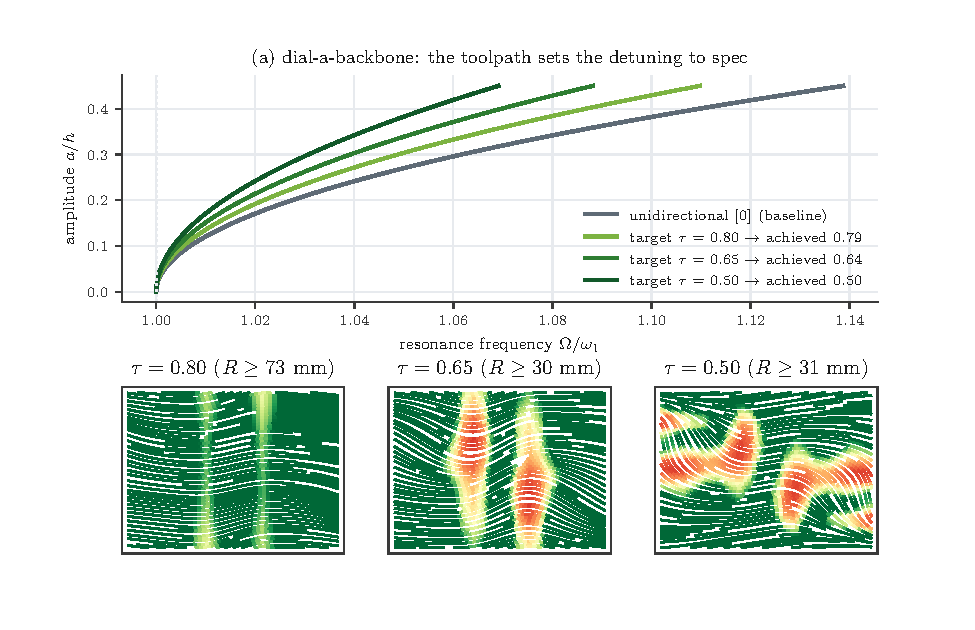
\includegraphics[width=\linewidth]{figs/plate_tune.pdf}
\caption{Designing the nonlinear response to a target. \emph{Top:} one panel's
first-mode backbone dialed to three prescribed relative detunings $\tau$ (a $20$--$50\%$
reduction), each landing on target at held frequency. \emph{Bottom:} the corresponding
fiber toolpaths, coloured by local steering radius --- a deeper target requires more
aggressive (but still feasible) steering.}
\label{fig:tune}
\end{figure}

\section{Two fields: topology \emph{and} fiber steering}\label{sec:topopt}

The orientation field decides which way the tows run; the second wavetopo design
field --- the structural \emph{density} $\bm z$ --- decides where material goes at
all. Adding it turns the problem into genuine topology optimization coupled to
fiber steering, and it plugs into the same SSM backbone objective.

\subsection{Three-field density and the density-weighted backbone}
We use the standard density parametrization: a raw variable $z_e\in[0,1]$ per
element, a linear \emph{filter} $\bm y_f=\bm P\bm z$ (radius $R_\rho$, imposing a
minimum feature size), a smooth \emph{Heaviside projection}
$y=\tfrac{\tanh(\beta\eta)+\tanh(\beta(y_f-\eta))}{\tanh(\beta\eta)+\tanh(\beta(1-\eta))}$
that crisps the topology toward $0/1$ as $\beta$ is continued upward, and a SIMP
interpolation $E(y)=\varepsilon+(1-\varepsilon)y^{p}$ ($p=3$) of the element
stiffness. Every element quadratic form of Sec.~\ref{sec:plate} is scaled by
$E_e$: the bending $K_b=\sum_e E_e\,k^b_e$, the raw cubic
$\mathrm{knl}=\sum_e E_e\,k^{nl}_e$, the in-plane stiffness
$\bm K_{\mathrm{in}}=\sum_e E_e\,\bm K^{\mathrm{in}}_e$ and the coupling
$\bm g=\sum_e E_e\,\bm g_e$, so the relaxed backbone coefficient
$\gamma_{\mathrm{eff}}=\mathrm{knl}-2\bm g^{\!\top}\bm K_{\mathrm{in}}^{-1}\bm g$
(Eq.~\eqref{eq:gammaeff}) becomes a function of \emph{both} fields. The modal mass
$M=\rho h\sum_e y_e A_e\phi_e^2$ scales linearly with the physical density, so the
linear frequency $\omega_1=\sqrt{K_b/M}$ is available for the constraint below.

\subsection{Coupled sensitivities}
The design vector is $(\bm z,\hat{\bm\theta})$ and the objective is again
$J=\gamma_{\mathrm{eff}}/K_b$. The orientation sensitivity is Eq.~\eqref{eq:gammaeffadj}
with each element term now carrying its weight $E_e$. The density sensitivity
threads the three-field chain: with $\bm u^\star=\bm K_{\mathrm{in}}^{-1}\bm g$,
\begin{equation}
\frac{\partial\gamma_{\mathrm{eff}}}{\partial E_e}
=k^{nl}_e-4\,\bm g_e^{\!\top}\bm u^\star+2\,\bm u^{\star\top}\bm K^{\mathrm{in}}_e\bm u^\star,
\qquad
\frac{\dd J}{\dd\bm z}=\bm P^{\!\top}\!\Big[\frac{\partial J}{\partial E}\,
\frac{\dd E}{\dd y}\,\frac{\dd y}{\dd y_f}\Big],
\label{eq:dzchain}
\end{equation}
where $\partial J/\partial E=\partial_E\gamma_{\mathrm{eff}}/K_b-\gamma_{\mathrm{eff}}K_b^{-2}k^b_e$,
$\dd E/\dd y=(1-\varepsilon)p\,y^{p-1}$ and $\dd y/\dd y_f$ is the Heaviside
derivative --- and the single adjoint solve $\bm u^\star$ is reused across every
$z_e$ and every $\hat\theta_j$. Both sensitivities are verified against central
finite differences to $\lesssim\!10^{-7}$; the orientation sensitivity also passes
the \emph{isotropy-annihilation} test --- setting the lamina stiffness isotropic
makes the tow angle inert and drives $\partial J/\partial\hat{\bm\theta}$ to
$\sim\!10^{-9}$, confirming the whole angular chain.

\subsection{Constrained optimization}
We drive $(\bm z,\hat{\bm\theta})$ with MMA under an augmented-Lagrangian for three
constraints: the per-element tow-curvature limit $\zeta_e^2\le\zall^2$ (orientation
only), a material-volume budget $\overline{y}=v_{\mathrm{all}}$ as an
\emph{equality} (a fixed budget --- without it the scale-near-invariant $J$ would
drive material trivially to zero), and a linear-frequency \emph{band}
$f_{\mathrm{lo}}\,\omega_1^{\mathrm{ref}}\le\omega_1\le f_{\mathrm{hi}}\,\omega_1^{\mathrm{ref}}$.
The band's \emph{ceiling} is essential: with a floor alone the optimizer discovers
the spurious low-density localized mode where the SIMP $\varepsilon$-stiffness with
vanishing mass sends $\omega_1\!\to\!\infty$ and $\gamma_{\mathrm{eff}}\!\to\!0$
trivially, giving a disconnected sliver design; the ceiling forbids it. Because the
$(1,1)$ mode is symmetric about both centre-lines we project $\bm z$ onto the
quarter-symmetric subspace, which selects the physical optimum over lopsided local
minima.

\subsection{Result}
Figure~\ref{fig:topopt} shows the converged two-field design at a held frequency
and a fixed $50\%$ material budget. The topology is connected and symmetric, and it
voids material exactly at the top- and bottom-edge midpoints --- the antinodes of the
membrane stretch $(\nabla w)^2$, where the hardening integrand
$\bm\varepsilon_{NL}^{\!\top}\bm A\bm\varepsilon_{NL}$ concentrates --- while keeping
the high-curvature centre that carries the frequency; the tows then steer
\emph{around} the voids, curl-feasibly. The first-mode backbone drift falls from
$17.1\%$ to $3.0\%$ ($-83\%$), extending the orientation-only lever.

\paragraph{Confirmation on the adapted mode.} A single fixed master mode cannot
reshape around the new voids, so one might expect it to over-credit topology. It
does not: transferring the optimized topology onto the \emph{real multi-mode}
plate --- SIMP-weighting its stiffness and mass at every quadrature point so the
eigenmode itself adapts to the perforations --- the SSM detuning reduction is
$82\%$, against the reduced model's $83\%$. The relative-detuning lever therefore
\emph{survives} mode adaptation; it is not a fixed-mode artifact. One caveat we
state plainly: the single-mode frequency is a loose proxy for the real multi-mode
frequency of a strongly-steered design (the tow field alone reads far stiffer on
the multi-mode plate, and the voids bring the frequency back to $0.94\times$
baseline), so the topology design's held-frequency rests on a cancellation rather
than a tight constraint --- constraining the real multi-mode frequency directly is
the refinement. The contribution here is that the framework carries \emph{both}
manufacturable fields --- orientation and topology --- on the same verified SSM
backbone objective and its adjoint, and that the topology lever holds up against
the adapted-mode ground truth.

\begin{figure}[t]
\centering
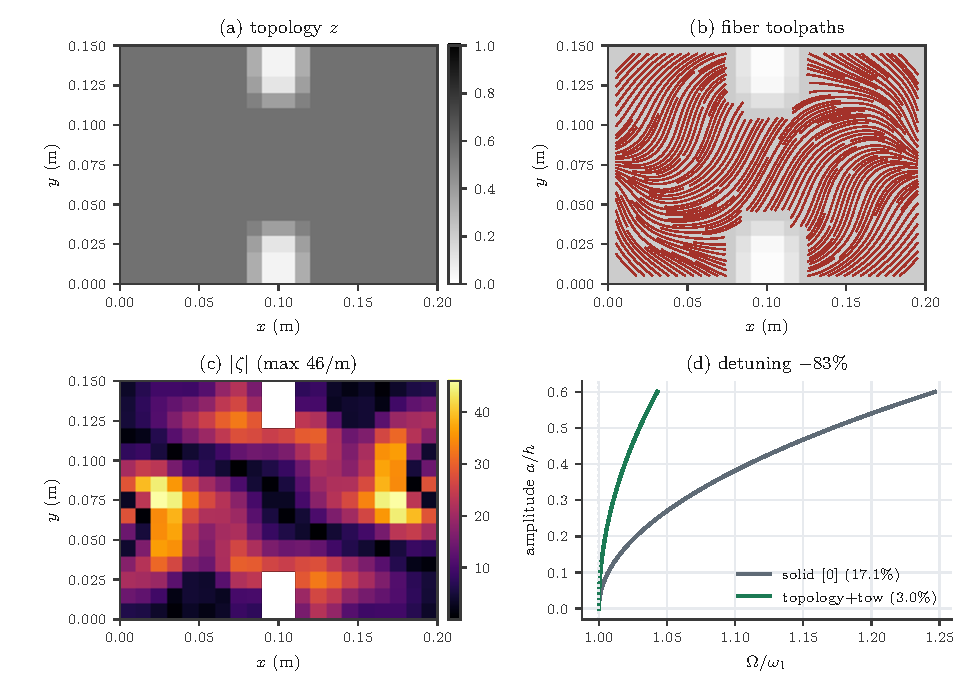
\includegraphics[width=\linewidth]{figs/plate_topopt.pdf}
\caption{Two-field (topology + fiber-steering) design of the nonlinear backbone,
rendered with wavetopo's tow/curl renderers. (a)~the converged composite topology
(density field $\bm z$); (b)~the manufacturable fiber toolpaths, masked to the solid
region and steering around the voids; (c)~the tow curl $|\zeta|$ (curl-feasible,
$R\ge22$\,mm); (d)~the first-mode backbone of the solid unidirectional plate (grey)
vs.\ the two-field design (green) at held frequency and fixed material budget ---
drift $17.1\%\!\to\!3.0\%$. The voids sit at the membrane-stretch antinodes (the
plate edges' midpoints), where the hardening integrand concentrates.}
\label{fig:topopt}
\end{figure}

\section{Designing the backbone to spec on the adapted mode}\label{sec:points}

The one caveat left standing (Sec.~\ref{sec:topopt}) was that a \emph{fixed} master
mode mistracks the linear frequency of a strongly-steered design. We close it with
a \emph{mode-adaptive} reduction and use it to design the backbone to a target.

\subsection{The adapted-mode reduction and its analytic gradient}
Rather than freeze the master mode, take it to be the fundamental of the multi-mode
Ritz eigenproblem $\bm K_b(\theta)\bm v=\omega_1^2\bm M\bm v$ over a small transverse
basis $\{\phi_k\}$; the mode $w=\sum_k v_k\phi_k$ then reshapes with the design and
$\omega_1$ is the \emph{real} multi-mode frequency. The relaxed cubic
$\gamma_{\mathrm{eff}}$ (Eq.~\eqref{eq:gammaeff}) is evaluated on this adapted mode,
and the objective is $J=\gamma_{\mathrm{eff}}/(\omega_1^2\,m_c^2)$ with $m_c$ the
mode's midspan value (which fixes the physical amplitude normalization). The
gradient is fully analytic and FD-verified to $\sim\!10^{-7}$: the eigenvalue
(frequency) sensitivity is Fox--Kapoor and needs no eigenvector derivative, while the
two eigenvector-sensitivity terms --- of $\gamma_{\mathrm{eff}}$ and of $m_c$ ---
each collapse to a \emph{single adjoint curvature field}
$\kappa_\beta=\sum_{j\ne0}\beta_j\,\kappa_{v_j}$, so the whole sensitivity costs the
one eigensolve plus cheap contractions.

\subsection{Threading the backbone through design points}
With both knobs in hand --- the real $\omega_1$ and the hardening curvature, each with
a verified gradient --- we can \emph{place} the backbone: minimizing the squared
mismatch to prescribed $(\,f_k,\,a_k)$ points in the frequency--amplitude plane steers
the tow field so the real backbone threads them. A caution the plate enforces: its
cubic backbone is a two-parameter family (a linear frequency and one hardening
curvature), so admissible design points must lie on \emph{one} achievable, positively
sloped hardening curve --- a vertical (iso-frequency-across-amplitude) target is not a
backbone a hardening plate can produce. Figure~\ref{fig:points} designs an
amplitude-stable resonator mandated near $335$ Hz: the toolpath threads three points
on a gentle-hardening target to an rms error of $3.3$ Hz ($\sim\!1\%$), curl-feasibly,
far flatter and higher than the unidirectional baseline. Crucially, the adapted-mode
frequency ($332$ Hz) agrees with the full multi-mode plate ($337$ Hz) to $1.5\%$ ---
where the old fixed-mode proxy erred by $70\%$ --- so the shipped device actually sits
at its mandated frequency. This is the manufacturable, frequency-honest version of
the response-curve design of \cite{pozzi2025,liang2025}.

\begin{figure}[t]
\centering
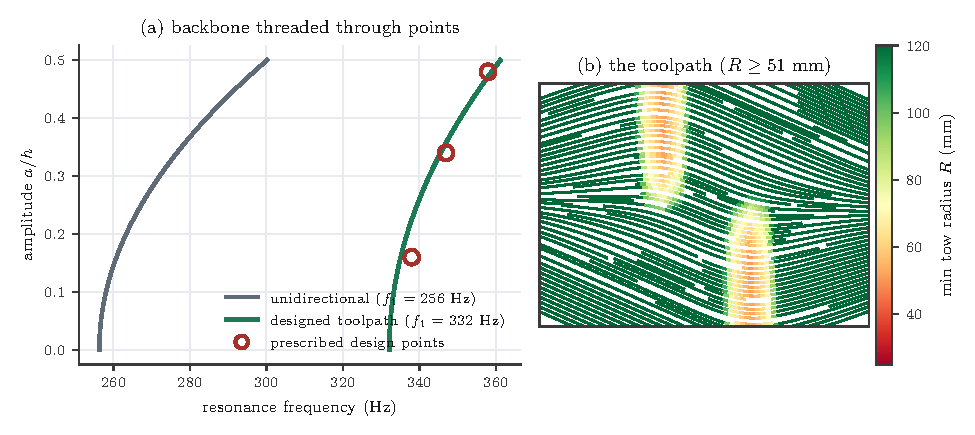
\includegraphics[width=\linewidth]{figs/plate_designpoints.pdf}
\caption{Designing a nonlinear backbone to spec. \emph{Left:} the tow field is steered
so the real (mode-adaptive) first-mode backbone threads three prescribed design points
(circles) on a gentle-hardening target at a mandated $\sim\!335$ Hz --- distinct from
the unidirectional baseline (grey, $256$ Hz, steep). \emph{Right:} the manufacturable
toolpath that does it, coloured by local steering radius. The reported frequency is the
real multi-mode value (within $1.5\%$ of the full plate), not a fixed-mode proxy.}
\label{fig:points}
\end{figure}

\section{Designing an instability boundary: supersonic panel flutter}\label{sec:flutter}

The backbone is one target the framework exposes; the \emph{same} machinery designs a
\emph{stability boundary}. A thin panel in supersonic flow loses stability by flutter --- a
Hopf bifurcation of the flat state into self-excited oscillation --- and keeping that boundary
above the flight envelope is a hard constraint on every high-speed skin panel. Fiber steering
is the natural manufacturable lever (this extends the variable-stiffness tailoring of
\cite{gurdal,ijsselmuiden} from linear objectives to a nonlinear instability), and the
geometric nonlinearity sets what happens \emph{past} the boundary.

\subsection{Aeroelastic model and calibration}
First-order piston theory gives the aerodynamic pressure on a panel in a stream of Mach
number $M_\infty$ and dynamic pressure $q$; projected on the transverse modes it adds a
\emph{nonsymmetric} aerodynamic stiffness (the streamwise slope term) to the bending block,
\begin{equation}
G_{ij}=\!\int_\Omega\!\phi_i\,\partial_x\phi_j\,\dd\Omega,\qquad
\bm M\ddot{\bm q}+\bm C\dot{\bm q}+\big(\bm K_b(\theta)+\lambda_q\bm G\big)\bm q=\bm 0,
\quad \lambda_q=\tfrac{2q}{\sqrt{M_\infty^2-1}},
\label{eq:flutter-eom}
\end{equation}
plus light damping $\bm C$. Equation~\eqref{eq:flutter-eom} is a nonsymmetric generalized
eigenproblem; as $q$ rises two modes coalesce in frequency and a complex-conjugate pair of the
first-order pencil crosses the imaginary axis at the critical $q_{\mathrm{cr}}$ ---
\emph{coalescence flutter}. The implementation reproduces the classical result: a
one-dimensional simply-supported panel gives the nondimensional critical dynamic pressure
$\lambda_{\mathrm{cr}}=343.35$ against the textbook $343.36$ \cite{shaw}.

\subsection{Conforming discretization: why the assumed modes fail here}\label{sec:flutter-fe}
Unlike the backbone, the flutter boundary is \emph{not} adequately resolved by the global sine
modes. A steered --- or merely rotated --- laminate develops bend--twist couplings $D_{16},D_{26}$
that \emph{twist} the mode shapes; flutter is a coalescence of two modes and is exquisitely sensitive
to their shape, and the sine basis, which cannot represent the twist, gives the wrong coalescence. We
established this against an independent \emph{conforming} Bogner--Fox--Schmit (BFS) bicubic-Hermite
Kirchhoff element (nodal DOF $w,w_{,x},w_{,y},w_{,xy}$; frequencies exact against the closed form as in
App.~\ref{app:fe}): the two discretizations \emph{agree} while $D_{16}\!\approx\!0$
($0^\circ$--$5^\circ$) and \emph{diverge monotonically} as the coupling grows --- by a factor of
\emph{ten} at $30^\circ$, where the sine model over-predicts $q_{\mathrm{cr}}$ tenfold. The flutter
results below therefore use the conforming BFS element, and the sine-mode flutter is discarded. (The
backbone results of Secs.~\ref{sec:plate}--\ref{sec:points} are unaffected: those are frequencies and
detuning \emph{ratios}, FE-accurate to $\sim\!2\%$, App.~\ref{app:fe}.)

\subsection{Steering the boundary out}
On the conforming model the flutter boundary is a strong, \emph{non-monotone} function of the ply
angle: bend--twist coupling is maximally destabilizing near $30^\circ$--$40^\circ$, where a uniform
CFRP panel's $q_{\mathrm{cr}}$ collapses into a ``flutter hole'' an order of magnitude below the
flow-aligned $[0]$ value (Fig.~\ref{fig:flutter}a). A required operating frequency that places a
uniform layup in that hole is exactly where steering helps: the linear frequency and the flutter
boundary read the tow field through different operators, so a steered \emph{field} can hold the
frequency while placing the twist where it stabilizes rather than destabilizes. We maximize
$q_{\mathrm{cr}}$ at held $f_1$ and mass, curl-feasibly, driving the search by the boundary's analytic
adjoint --- the implicit eigenvalue derivative
\begin{equation}
\frac{\dd q_{\mathrm{cr}}}{\dd\theta}=-\frac{\mathrm{Re}(\dd s/\dd\theta)}{\mathrm{Re}(\dd s/\dd q)},
\qquad
\frac{\dd s}{\dd p}=\frac{\bm u^{*}(\partial_p\bm{\mathcal A})\,\bm v}{\bm u^{*}\bm{\mathcal B}\,\bm v},
\label{eq:flutter-adj}
\end{equation}
with $\bm u,\bm v$ the left/right eigenvectors of the critical mode of the (reduced) nonsymmetric
aeroelastic pencil --- the same left-eigenvector projection as the SSM adjoint (Eq.~\eqref{eq:gamma}),
the reduction being built on a general pencil that never assumed self-adjointness. Formed on the
conforming FE (reduced on its own modes, the modal-basis sensitivity absorbed by refreshing the basis
each design step), it is FD-verified to $2.1\times10^{-7}$. On a $200\times150\times2\,\si{mm}$ CFRP
panel at $M_\infty=2$ and a held $f_1=300\,\si{Hz}$ --- where the best uniform layup flutters at only
$\sim\!0.37\,\si{MPa}$ --- a curl-feasible steered field \textbf{recovers the flutter boundary to
$3.4\,\si{MPa}$, a $9\times$ margin} at held frequency and mass
(Figs.~\ref{fig:fluttermech}b, \ref{fig:flutter}b). Steering pushes the bending--torsion coalescence
from $q_{\mathrm{cr}}=0.37$ to $3.4\,\si{MPa}$ (Fig.~\ref{fig:fluttermech}a), sliding the growth-rate
zero-crossing --- the Hopf onset --- the same $9\times$ to the right (Fig.~\ref{fig:fluttermech}b). The
lever is the manufacturable placement of the same bend--twist coupling that, uncontrolled, craters the
uniform panel.

\begin{figure}[t]
\centering
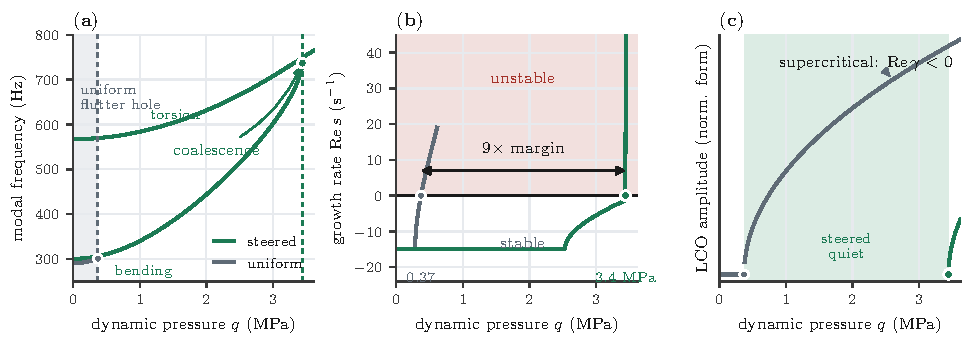
\includegraphics[width=\linewidth]{figs/plate_flutter_mechanism.pdf}
\caption{How steering reshapes the aeroelastic response of the panel (conforming BFS pencil; the best
uniform layup at $300\,\si{Hz}$ vs.\ the steered field). \emph{(a)}~modal frequency vs.\ dynamic
pressure: the steered layup's bending and torsion branches coalesce far out in $q$ (classic coalescence
flutter, $745\,\si{Hz}$), whereas the uniform ``flutter-hole'' layup loses a single mode early.
\emph{(b)}~growth rate $\mathrm{Re}\,s$ of the critical mode crosses zero --- the Hopf onset --- at
$q_{\mathrm{cr}}$; steering slides that crossing $\sim\!9\times$ to higher $q$ at held frequency and
mass. \emph{(c)}~past the boundary $\mathrm{Re}\,\gamma<0$ makes the Hopf supercritical, so the panel
settles into a bounded limit cycle ($a\!\sim\!\sqrt{q-q_{\mathrm{cr}}}$, normal form); the shaded band is
the recovered margin over which the steered panel stays quiet.}
\label{fig:fluttermech}
\end{figure}

\begin{figure}[t]
\centering
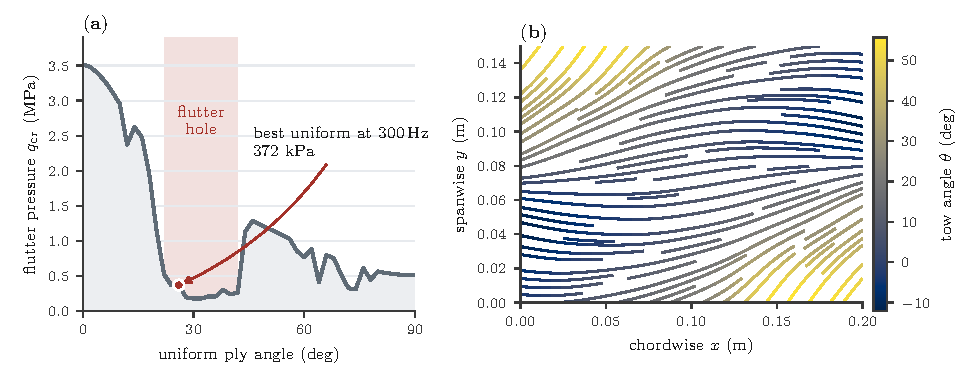
\includegraphics[width=\linewidth]{figs/plate_flutter.pdf}
\caption{Flutter boundary on the conforming BFS FE. \emph{(a)}~the boundary vs.\ uniform ply angle
collapses into a bend--twist ``flutter hole'' near $30^\circ$--$40^\circ$ (where $D_{16}$ peaks), an
order of magnitude below the flow-aligned value, so the best uniform layup that reaches the required
$300\,\si{Hz}$ flutters at only $\sim\!0.37\,\si{MPa}$. \emph{(b)}~the manufacturable steered tow field
that recovers the boundary to $3.4\,\si{MPa}$ at held frequency and mass.}
\label{fig:flutter}
\end{figure}

\subsection{The nonlinear aftermath}
Past the boundary the geometric nonlinearity sets the consequence. Restoring the von~K\'arm\'an
relaxed cubic and reducing the flutter mode onto its Stuart--Landau normal form
$\dot p=\lambda(q)\,p+\gamma\,p|p|^2$, the cubic coefficient --- formed from the same left/right
flutter eigenvectors and the von~K\'arm\'an cubic tensor by the $\bm u_1^{*}$ projection --- has
$\mathrm{Re}\,\gamma<0$: the Hopf is \emph{supercritical}, so crossing it yields a benign, bounded
limit-cycle oscillation rather than a catastrophic subcritical jump (Fig.~\ref{fig:fluttermech}c). This criticality --- the sign of
$\mathrm{Re}\,\gamma$ --- is the cheap, model-robust output of the reduction. The finite limit-cycle
amplitude on the conforming model, and its reduction by steering, are a direct follow-on (our earlier
assumed-modes limit-cycle amplitudes are superseded along with the boundary they rested on).

\subsection{Relation to the framework}
Flutter uses no new reduction machinery --- the nonsymmetric aerodynamic operator drops into the same
first-order pencil, and the boundary sensitivity~\eqref{eq:flutter-adj} is the same left-eigenvector
projection as the backbone adjoint --- but it did force a \emph{conforming} discretization, and that
rigor is the point: an independent FE cross-check overturned a plausible-looking sine-mode result and
replaced a spurious $2\times$ with a correct, larger $9\times$ recovery. Linear flutter tailoring is
itself classical aeroelasticity; the contribution here is its manufacturable, adjoint-driven form on a
discretization honest enough to trust.


\begin{thebibliography}{99}
\bibitem{haller2016} G.\ Haller and S.\ Ponsioen, ``Nonlinear normal modes and
spectral submanifolds: existence, uniqueness and use in model reduction,''
\emph{Nonlinear Dyn.} \textbf{86}(3), 1493--1534, 2016.
\bibitem{jain2022} S.\ Jain and G.\ Haller, ``How to compute invariant manifolds
and their reduced dynamics in high-dimensional finite element models,''
\emph{Nonlinear Dyn.} \textbf{107}, 1417--1450, 2022.
\bibitem{pozzi2025} M.\ Pozzi, J.\ Marconi, S.\ Jain, M.\ Li, F.\ Braghin,
``Adjoint sensitivities for the optimization of nonlinear structural dynamics
via spectral submanifolds,'' 2025 (arXiv:2503.17431).
\bibitem{liang2025} H.\ Liang, M.\ Pozzi, J.\ Marconi, S.\ Jain, M.\ Li,
``Topology optimization of nonlinear forced response curves via reduction on
spectral submanifolds,'' 2025 (arXiv:2510.07900).
\bibitem{xiao2026} X.\ Xiao, ``Using reduced-order models to optimise the
dynamics of nonlinear systems,'' PhD thesis, University of Bristol, 2026.
\bibitem{li2024} M.\ Li, ``Explicit sensitivity analysis of spectral submanifolds
of mechanical systems,'' \emph{Nonlinear Dyn.}, 2024.
\bibitem{krack2015} M.\ Krack, ``Nonlinear modal analysis of nonconservative
systems: extension of the periodic motion concept,'' \emph{Computers \& Structures}
\textbf{154}, 59--71, 2015.
\bibitem{shaw} S.\,W.\ Shaw and C.\ Pierre, ``Normal modes for non-linear
vibratory systems,'' \emph{J.\ Sound Vib.} \textbf{164}(1), 85--124, 1993.
\bibitem{touze} C.\ Touz\'e, A.\ Vizzaccaro, O.\ Thomas, ``Model order reduction
methods for geometrically nonlinear structures,'' \emph{Nonlinear Dyn.}
\textbf{105}, 1141--1190, 2021.
\bibitem{gurdal} Z.\ G\"urdal, B.\,F.\ Tatting, C.\,K.\ Wu, ``Variable stiffness
composite panels: effects of stiffness variation on the in-plane and buckling
response,'' \emph{Composites A} \textbf{39}(5), 911--922, 2008.
\bibitem{ijsselmuiden} S.\,T.\ IJsselmuiden, M.\,M.\ Abdalla, Z.\ G\"urdal,
``Optimization of variable-stiffness panels for maximum buckling load using
lamination parameters,'' \emph{AIAA J.} \textbf{48}(1), 134--143, 2010.
\end{thebibliography}
\end{document}
